\documentclass{article}

\usepackage[utf8x]{inputenc}
\usepackage[english,russian]{babel}
\usepackage{cmap}
\usepackage{commath}
\usepackage{amsmath}
\usepackage{amsfonts}
\usepackage{mathtools}
\usepackage{amssymb}
\usepackage{parskip}
\usepackage{titling}
\usepackage{color}
\usepackage{hyperref}
\usepackage{cancel}
\usepackage{enumerate}
\usepackage{multicol}
\usepackage{graphicx}
\usepackage[font=small,labelfont=bf]{caption}
\usepackage[a4paper, left=2.5cm, right=1.5cm, top=2.5cm, bottom=2.5cm]{geometry}

\graphicspath{ {./images/} }
\setlength{\droptitle}{-3cm}
\hypersetup{ colorlinks=true, linktoc=all, linkcolor=blue }
\pagenumbering{arabic}

\begin{document}


    \textbf{Теорема 1. (производная сложной функции)}

    \( y = f(u), u = \varphi(x) \) имеют производную, \( \exists y= F(x) = f(\varphi(x)) \), тогда \( F'(x) = f_u'(\varphi(x)) \cdot \varphi_x'(x) \)\\
    \( \uparrow \)
    
    \(x\) придали приращение \(\Delta x\); то \(u\) получила приращение \(\Delta u = \varphi(x + \Delta x) - \varphi(x)\), тогда \(y\) получила приращение \(\Delta y = f(u + \Delta u) - f(u) \).
    
    \(\exists f_u\), т.е. \( f_u' = \lim_{\Delta u \to 0} \frac{\Delta y}{\Delta u} \Rightarrow \frac{\Delta y}{\Delta u} = f_u' + \alpha(\Delta u); \alpha(\Delta u) \xrightarrow[\Delta u \to 0]{} 0\)
    
    \(\Delta y = f_u'\Delta u + \alpha(\Delta u)\Delta u\)

    \( F'(x) = \lim_{\Delta x \to 0}\frac{\Delta y}{\Delta x} = \lim_{\Delta x \to 0} [f_u'\frac{\Delta u}{\Delta x} + \alpha(\Delta u)\frac{\Delta u}{\Delta x}] = f_u'(\varphi(x)) \cdot \varphi_x'(x) + 0 \cdot \varphi'(x) \), т.к. если \( \Delta x \to 0 \), то \(\Delta u \to 0\) (непр.) \( \Rightarrow \alpha(\Delta u) \to 0 \).
    \(\downarrow\)

    \textbf{Теорема 2. (производная обратной функции)}

    Пусть \( y = f(x) \) монотонна, непрерывна и \(\exists\) обратная функция \( x = f^{-1}(y) = g(y) \). Если при этом \(y'\Bigr|_{\substack{x_0}} = f'(x_0) \neq 0\) и конечна, тогда \(\exists\) производная \( g'(y) \) в \(y_0 = f(x_0)\) и при этом \(g'(y)\Bigr|_{\substack{y_0}} = \frac{1}{f_x'(g(y))\Bigr|_{\substack{y_0}}} \)

    \(\uparrow\)
    
    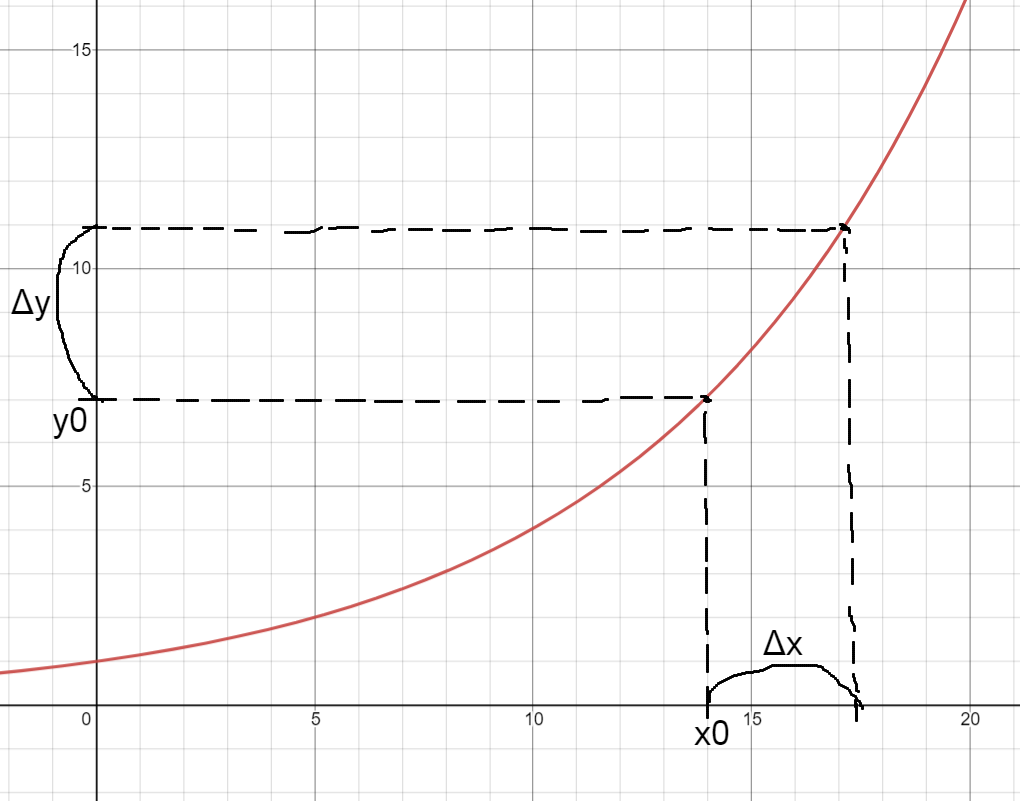
\includegraphics[scale=0.3]{11_1_9_1.png}

    Если \( \Delta y \neq 0 \), то \(\Delta x\)(соответствует этому \(\Delta y\)) \(\neq 0\), \(\Delta y \to 0\), то \(\Delta x \to 0\), т.к. \(g(y)\) --- непрерывна как обратная к непрерывной. 

    \(\frac{\Delta x}{\Delta y} = \frac{1}{\frac{\Delta y}{\Delta x}}\)

    \( g'(y)\Bigr|_{\substack{y_0}} = \lim_{\Delta y \to 0} \frac{\Delta x}{\Delta y} = \lim_{\Delta x \to 0} \frac{1}{\frac{\Delta y}{\Delta x}} = \frac{1}{f_x'(g(y))\Bigr|_{\substack{y_0}}} \)
    \(\downarrow\)

    \textbf{Примеры.}

    \begin{enumerate}
        \item \( y = a^x \)
        
        \( x = \log_a y \)

        \( x' = \frac{1}{y\ln a} \)

        \( y_x'(x) = \frac{1}{\frac{1}{y\ln a}} = y\ln a = a^x\ln a\)

        \( (a^x)' = a^x\ln a \)

        \begin{enumerate}
            \item \( y = e^x \)
            
            \( (e^x)' = e^x\ln e = e^x \)
        \end{enumerate}

        \item \( y = x^\alpha,\ \alpha \in \mathbb{R} \)
        
        \( y' = (x^\alpha)' = \alpha x^{\alpha - 1} \)

        \( (x^\alpha)' = (e^{\ln x^\alpha})' = (e^{\alpha\ln x})' = e^{\alpha\ln x} \cdot (\alpha\ln x)' = e^{\ln x^\alpha}(\alpha\frac{1}{x}) = x^\alpha \cdot \alpha \cdot \frac{1}{x} = \alpha x^{\alpha - 1} \)

        \item \( y = arctg(x), \frac{-\pi}{2} < y < \frac{\pi}{2}, tg(y) = x \)
        
        \( (arctg(x))' = \frac{1}{(tg y)'} = \frac{1}{\frac{1}{cos(y)^2}} = cos(y)^2 = \frac{1}{1 + tg(y)^2} = \frac{1}{1 + x^2} \)
        
    \end{enumerate}
    \begin{center}
        Таблица производных\\
        \begin{tabular}{ |c|c| }
            \hline
            \( y = f(x) \) & \( y' \) \\
            \hline
            \( c = const \) & \( 0 \)\\            
            \( x \) & \( 1 \)\\
            \( cx,\ c = const \) & \( c \)\\
            \( x^\alpha \) & \( \alpha x^{\alpha - 1} \)\\
            \( \sqrt{x} \) & \( \frac{1}{2\sqrt(x)} \)\\
            \( e^x \) & \( e^x \)\\
            \( a^x \) & \( a^x\ln a \)\\
            \( \ln x \) & \( \frac{1}{x} \)\\
            \( \log_a x \) & \( \frac{1}{x\ln a} \)\\
            \( sin(x) \) & \( cos(x) \)\\
            \( cos(x) \) & \( -sin(x) \)\\
            \( tg(x) \) & \( \frac{1}{cos(x)^2} \)\\
            \( ctg(x) \) & \( \frac{-1}{\sin(x)^2} \)\\
            \( arctg(x) \) & \( \frac{1}{1 + x^2} \)\\
            \( arcctg(x) \) & \( \frac{-1}{1 + x^2} \)\\
            \( arcsin(x) \) & \( \frac{1}{\sqrt{1 - x^2}} \)\\
            \( arccos(x) \) & \( \frac{-1}{\sqrt{1 - x^2}} \)\\
            \hline
        \end{tabular}
    \end{center}

    \subsection{Производная второго порядка и производные высших порядков}

    \( f(x) \) на \((a, b)\) (или на \([a, b]\)) и нашли \( f'(x) \) в каждой точке, т.е. \(f''(x) \stackrel{\text{df}}{=} (f'(x))' \)

    \textbf{Пример.} \( y = x^3; y' = 3x^2; y'' = 3\cdot 2x = 6x\)

    \textbf{Определение.} \( f^{(n)}(x) \stackrel{\text{df}}{=} [f^{(n - 1)}(x)]' \)

    \textbf{Пример.} \( y = x^m \)

    \begin{enumerate}
        \item \( y' = mx^{m - 1} \)
        \item \( y'' = (m)(m - 1)x^{m - 2} \)
        \item \( y''' = (m)(m - 1)(m - 2)x^{m - 3} \)
        \item \( y^{IV} = (m)(m - 1)(m - 2)(m - 3)x^{m - 4} \)
        \item[\(n\).] \( y^{(n)} = (m)(m - 1)...(m - (n - 1))x^{m - n}\) при \(n < m\)
        
        Если \(n = m: y^{(n)} = m!\) 

        Если \(n > m: y^{(n)} = 0\)
    \end{enumerate}

    \subsection{Дифференциал функции}

    \( y = f(x) \)    

    \( y' = f(x) = \lim_{\Delta x \to 0}\frac{\Delta y}{\Delta x} = \lim_{\Delta x \to 0}\frac{f(x + \Delta x) - f(x)}{\Delta x} \)

    \( \frac{\Delta y}{\Delta x} = f'(x) + \alpha(\Delta x);\ \alpha(\Delta x) \xrightarrow[\Delta x \to 0]{} 0\)

    \( \Delta y = f'(x)\Delta x + \alpha(\Delta x)\Delta x = f'(x)\Delta x + o(\Delta x) \), где \(f'(x)\Delta x\) --- линейно по \(\Delta x\), а \(\alpha(\Delta x)\Delta x \xrightarrow[\Delta x \to 0]{} 0\)

    \textbf{Пример.} \( y = x^2 \)

    \( \Delta y = (x + \Delta x)^2 - x^2 = 2x\Delta x + (\Delta x)^2 \)

    \( \lim_{\Delta x \to 0}\frac{\alpha(\Delta x)\Delta x}{\Delta x} = 0 \), т.е. \(\alpha(\Delta x)\Delta x\) --- величина бесконечно малая более высокого порядка, чем \(\Delta x\) их обозначают \(o(\Delta x)\) (читается как о-малое).

    \textbf{Определение.} Если приращение функции \( y = f(x) \) представимо в виде: (в некоторой точке \(x\)) \( \Delta y = A(x)dx + o(dx) \)(*), где \( dx = \Delta x \), то главная линейная часть приращения, т.е. \(A(x)\cdot dx\) называется дифференциалом \(dy = A(x)\cdot dx\), а функция \( y = f(x) \) называется дифференцируемой.

    \textbf{Пример.} \( y = x^2 \)

    \( \Delta y = 2x\Delta x + (\Delta x)^2 \)

    \( \lim_{\Delta x \to 0} \frac{(\Delta x)^2}{\Delta x} = 0 \)

    \( dy = 2xdx \)
    
    Можно назвать \( y = x^2 \) дифференцируемой.

    \textbf{Теорема.} Для того, чтобы функция \( y = f(x) \) имела дифференциал в точке \(x\) необходимо и достаточно, чтобы \(\exists f'(x)\) в т. \(x\).

    \(\uparrow\)

    ``\( \Rightarrow \)'' т.е. \( \Delta y \) представимо в виде: \( \Delta y = A(x)dx + o(dx) \)

    \(f'(x) = \lim_{\Delta x \to 0}\frac{\Delta y}{\Delta x} = \lim_{\Delta x \to 0}\frac{A(x)\Delta x + o(\Delta x)}{\Delta x} = A(x) + 0 \)

    ``\( \Leftarrow \)'' \(\exists f'(x) \Rightarrow\ \exists \) представление для \(\Delta y\) вида (*), где \(A(x) = f'(x) \downarrow\).

    \subsubsection{Геометрический смысл дифференциала}

    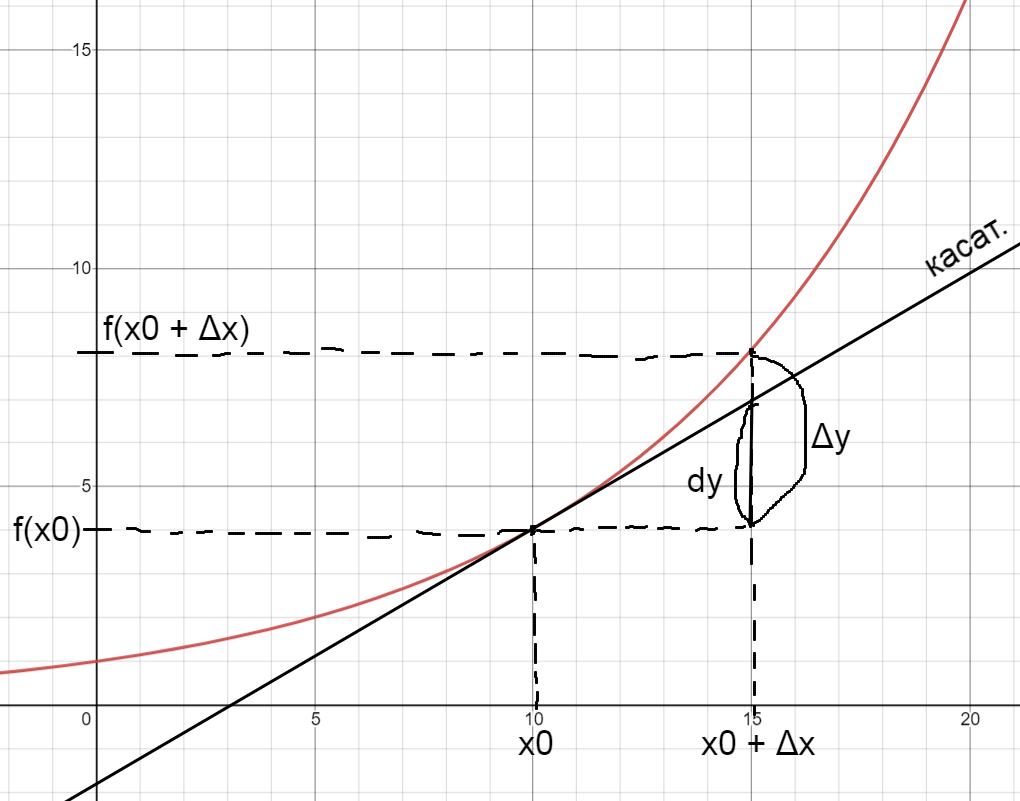
\includegraphics[scale=0.3]{11_1_9_2.png}

    \( y_{\textrm{кас}} = f'(x)(x - x_0) + f(x_0) \)

    \( y_{\textrm{кас}} - f(x_0) = f^{\Delta x'}(x_0)(x - x_0) = dy\Bigr|_{\substack{x_0}} \)

    \( \Delta x \to 0: dy \approx \Delta y \)

    \textbf{Внимание.} Дифференциал \(\neq\) производная.

    \subsubsection{Использование.}

    \textbf{Приближенные вычисления}

    \( \sqrt{4.02} \)

    \( y = \sqrt{x},\ x = 4\)
    
    \( dy = \frac{1}{2\sqrt{x}}dx,\ dx = \Delta x = 0.02 \)

    \( \Delta y = \sqrt{4 + 0.02} - \sqrt{4} \approx \frac{1}{2\sqrt{4}}0.02 \)

    \( \sqrt{4.02} \approx \sqrt{4} + \frac{0.02}{4} = 2 + \frac{0.01}{2} = 2.005 \)

    \subsubsection{Свойства.}

    \begin{enumerate}
        \item[\(0\).] Инвариантность формы 1-го дифференциала.
        
        \( y = f(x),\ dy = f'(x)dx \), где \( dx = \Delta x \).

        \begin{enumerate}
            \item Естественно
            
            \( y = x,\ dx = dy = 1\cdot \Delta x \)
            
            \item Удобно 
            
            Т.к. форма дифференциала сохраняется вне зависимости от того, является ли \(x\) независимой от переменной (какая-то функция) или это промежуток.

            \( x = \varphi(t),\ y = f(x) = F(t) = F(\varphi(t)) \)

            \( dy = F_t'(t)dt = f_x' \cdot \varphi_t'dt = f_x'dx \)

            Если бы мы оставили 

            \( dy = f_x'(x)\Delta x \)(**)

            \( \Delta x = \varphi(t + \Delta t) - \varphi(t) \)

            \( \exists \lim_{\Delta t \to 0}\frac{\Delta x}{\Delta t} = \varphi_t'(t) \Rightarrow \Delta x = \varphi_t' \cdot \Delta t + \alpha(\Delta t)\cdot\Delta t \), если это подставить в (**), то \( dy = f_x'\varphi_t'\Delta t + f_x'\alpha(\Delta t)\Delta t = F_t'\Delta t + f_x'\alpha(\Delta t)\Delta t \)

            % Должно было получиться \( dy = F_t'\Delta t \),
        \end{enumerate}

        \item \( d(u \pm v) = du \pm dv \)
        \item \( d(uv) = vdu + udv \) 
        \item \( d(\frac{u}{v}) = \frac{vdu - udv}{v^2} \)


    \end{enumerate}

\end{document}
